%!TEX root = ../report.tex

\begin{figure}[H]
    \newcommand{\figurewidth}{0.5\textwidth}
    \newcommand{\figureheight}{5cm}
	\begin{subfigure}[b]{\figurewidth}
        \centering
        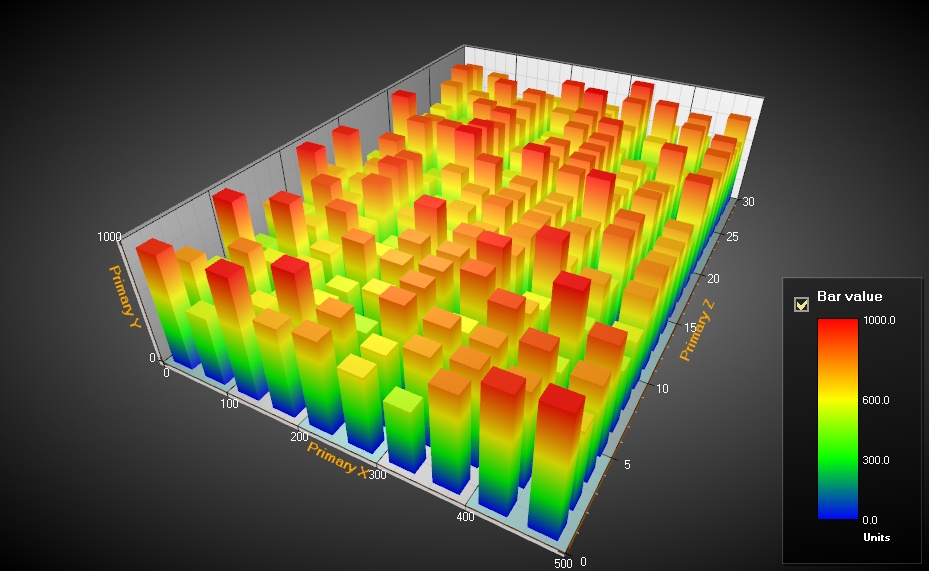
\includegraphics[width=\textwidth,height=\figureheight]{images/introduction/financial}
        \caption{A heat map of financial data. \protect\footnotemark}
        \label{fig:heat_map_financial}
    \end{subfigure}
    \begin{subfigure}[b]{\figurewidth}
        \centering
        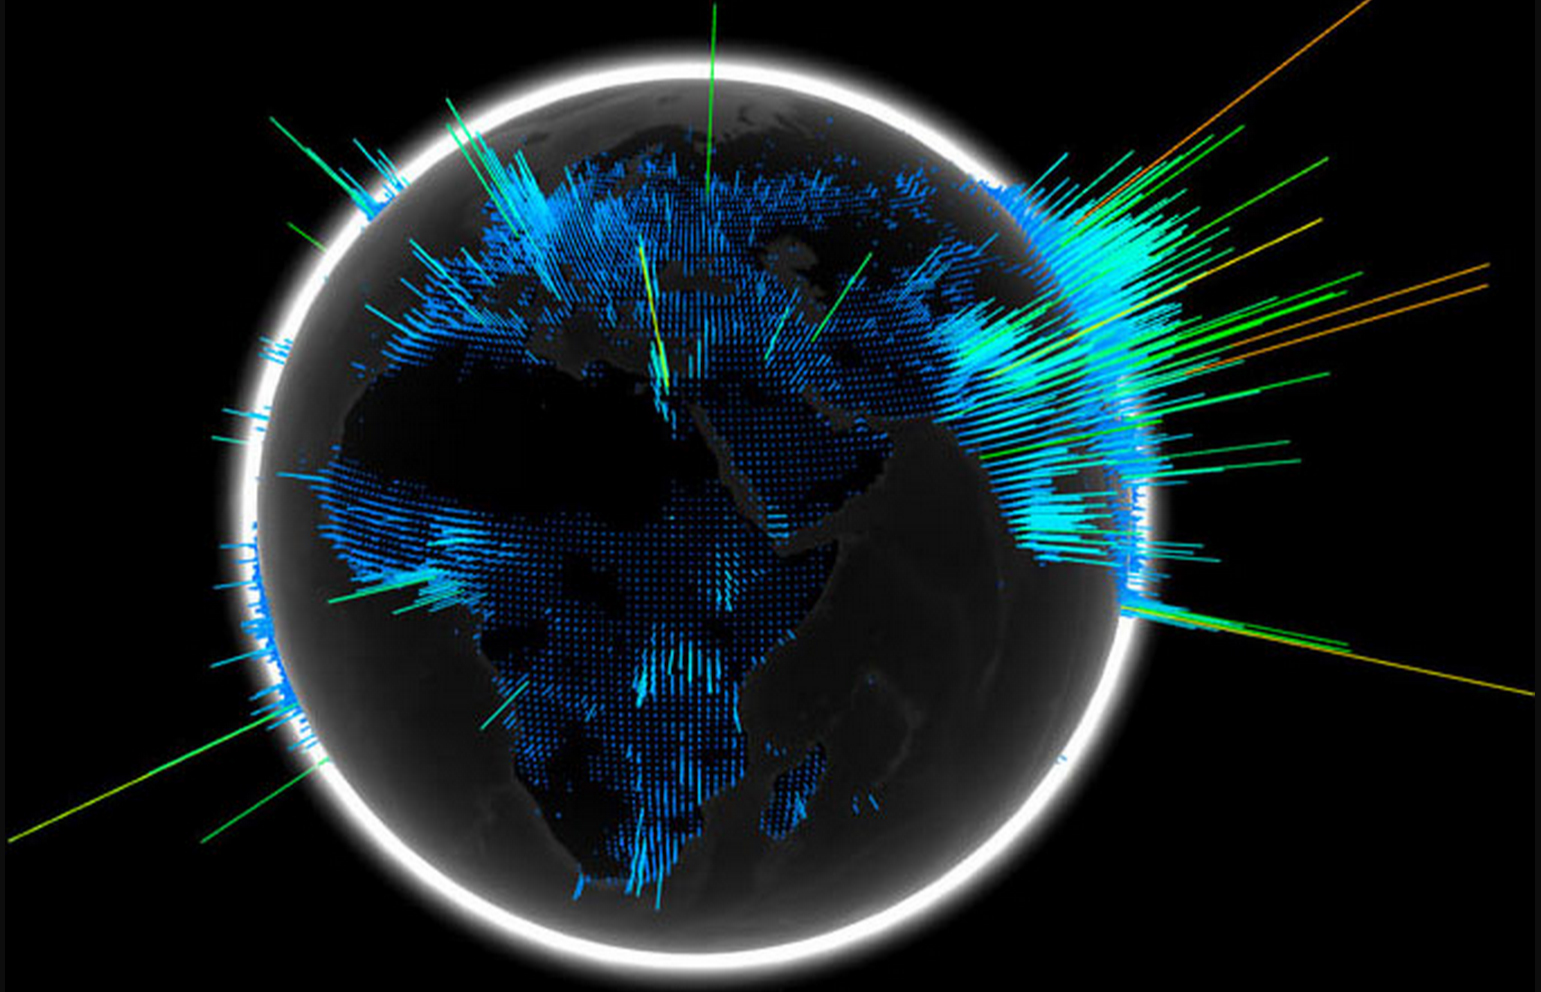
\includegraphics[width=\textwidth,height=\figureheight]{images/introduction/globe}
        \caption{WebGL globe. \protect\footnotemark}
        \label{fig:webgl_globe}
    \end{subfigure}
	\caption[3D representations]{Two different ways of representing 3D data.}
	\label{fig:3d_representations}
\end{figure}

\addtocounter{footnote}{-2}
\stepcounter{footnote}\footnotetext{\bibentry{tuomainen2014financial}}
\stepcounter{footnote}\footnotetext{\bibentry{google2011globe}}
